\documentclass{article}
\usepackage{graphicx}
\usepackage[margin=1in]{geometry}
\usepackage[outdir=./]{epstopdf}  					% Avoids errors when input figures
\usepackage[labelsep=period,labelfont=bf]{caption}
%\usepackage{subcaption}

\begin{document}
	\begin{figure}[tbph]
		\caption{Response of 2-Year U.S. Yield to U.S. Monetary Policy Surprises} \label{fig:LPUS2Y}
		\begin{center}
			\begin{minipage}{\linewidth}
				\begin{center}
					\begin{subfigure}[t]{\linewidth}
						\includegraphics[trim={0cm 0cm 0cm 0cm},clip,height=0.24\textheight,width=\linewidth]{../Figures/LPs/LagDep-FX/Target/US/DCMP/TargetUSDnomyptp24m.eps} \\
						\vspace{-0.35cm}
						\caption{Target Surprise: 2000-2008} \label{subfig:LPUS2Ytarget}
						\vspace{0.4cm}
					\end{subfigure}
					
					\begin{subfigure}[t]{\linewidth}
						\includegraphics[trim={0cm 0cm 0cm 0cm},clip,height=0.24\textheight,width=\linewidth]{../Figures/LPs/LagDep-FX/Path/US/DCMP/PathUSDnomyptp24m.eps} \\
						\vspace{-0.35cm}
						\caption{Forward Guidance Surprise: 2000-2019} \label{subfig:LPUS2Ypath}
					\end{subfigure}
					
					\begin{subfigure}[t]{\linewidth}
						\includegraphics[trim={0cm 0cm 0cm 0cm},clip,height=0.24\textheight,width=\linewidth]{../Figures/LPs/LagDep-FX/LSAP/US/DCMP/LSAPUSDnomyptp24m.eps} \\
						\vspace{-0.35cm}
						\caption{Asset Purchase Surprise: 2009-2019} \label{subfig:LPUS2Ylsap}
					\end{subfigure}
				\end{center}
				\fignotes{This figure shows the response following \cite{Jorda:2005} of the 2-year U.S. yield and its components to U.S. monetary policy surprises. The U.S. yield is the zero coupon yield from \cite{GSW:2007}. The yield is decomposed into an expected future short-term interest rate and a term premium following \cite{KimWright:2005}. The target, forward guidance and asset purchase surprises are identified using high-frequency data around Fed's monetary policy announcements, see section \ref{sec:USMPS} for details.}
			\end{minipage}
		\end{center}
	\end{figure}

	\pagebreak[4]
	
	\begin{figure}[tbph]
		\caption{Response of 10-Year U.S. Yield to U.S. Monetary Policy Surprises} \label{fig:LPUS10Y}
		\begin{center}
			\begin{minipage}{\linewidth}
				\begin{center}
					\begin{subfigure}[t]{\linewidth}
						\includegraphics[trim={0cm 0cm 0cm 0cm},clip,height=0.24\textheight,width=\linewidth]{../Figures/LPs/LagDep-FX/Target/US/DCMP/TargetUSDnomyptp120m.eps} \\
						\vspace{-0.35cm}
						\caption{Target Surprise: 2000-2008} \label{subfig:LPUS10Ytarget}
						\vspace{0.4cm}
					\end{subfigure}
					
					\begin{subfigure}[t]{\linewidth}
						\includegraphics[trim={0cm 0cm 0cm 0cm},clip,height=0.24\textheight,width=\linewidth]{../Figures/LPs/LagDep-FX/Path/US/DCMP/PathUSDnomyptp120m.eps} \\
						\vspace{-0.35cm}
						\caption{Forward Guidance Surprise: 2000-2019} \label{subfig:LPUS10Ypath}
					\end{subfigure}
					
					\begin{subfigure}[t]{\linewidth}
						\includegraphics[trim={0cm 0cm 0cm 0cm},clip,height=0.24\textheight,width=\linewidth]{../Figures/LPs/LagDep-FX/LSAP/US/DCMP/LSAPUSDnomyptp120m.eps} \\
						\vspace{-0.35cm}
						\caption{Asset Purchase Surprise: 2009-2019} \label{subfig:LPUS10Ylsap}
					\end{subfigure}
				\end{center}
				\fignotes{This figure shows the response following \cite{Jorda:2005} of the 10-year U.S. yield and its components to U.S. monetary policy surprises. The U.S. yield is the zero coupon yield from \cite{GSW:2007}. The yield is decomposed into an expected future short-term interest rate and a term premium following \cite{KimWright:2005}. The target, forward guidance and asset purchase surprises are identified using high-frequency data around Fed's monetary policy announcements, see section \ref{sec:USMPS} for details.}
			\end{minipage}
		\end{center}
	\end{figure}
\end{document}
% trim = {<left> <lower> <right> <upper>}